% Syntax for images is:
%\begin{figure}[h!]
%\centering
%\includegraphics{}
%\caption{}
%\label{}
%\end{figure}

% Intro											% ----

% What did I want to test?
% Predictions/baseline.


%TODO: update this
In this chapter, I will describe the experiments I performed to evaluate \mbt. There are 4 parameters that I will be altering, they are:
\begin{enumerate}
\item The thinking time available for the MCTS algorithm. 
\item The presence/absence of the two different opponent models. 
\item The selection strategy.
% being used and its parameters.
\item The number of opponents.
%\item The type of the opponent (\sbt or another poker bot).
\end{enumerate}

%In this chapter I will be varying each of these factors to see what effects they have on the performance and play style of \mbt.


\section{Experimental Setup}					% ----

% Producing the graphs and the Exporter class. 
% Why \sbt?
% Default settings?
% Clarify what is meant by performance.
% There are a total of 53488 games played by \sbt.

% TODO: write a brief intro, talk about the default values used and my machine specs.

%Before I get started with the evaluation, I will briefly explain the experimental setup that I used.

% Doesn't sound right.
% First, I made the necessary changes in the \mbt source code and exported a new jar file to the location required by \pa. I then started \pa and created a game between \mbt and \sbt (or other opponents if needed). I started the game and let it run overnight. In the morning, I stopped the game and exported the hand histories. Because I had already made a class to convert the hand histories, I used it again to calculate the profit per hand and write that to a file. I then created the graphs using a program called rlplot. Everything was done on the same computer for consistency.\footnote{The specs of the computer are: Quad Core 2.4GHz CPU ; 3GB RAM; running Windows~7. However the program is only single threaded so only one core was being used. I also noticed that the CPU was almost always the limiting factor.}


To perform most of these experiments, I played \mbt against \sbt in \pap and exported the hand histories. Because I had already made a class to convert the hand histories, I used it again to calculate the profit per hand and write it to a file. I created the graphs using a program called rlplot. Everything was done on the same computer for consistency\footnote{The specs of the computer are: Quad Core 2.4GHz CPU ; 3GB RAM; running Windows~7. However the program is only single threaded so only one core was being used. I also noticed that (one core of) the CPU was almost always at maximum utilization and so was probably the limiting factor.}.

Unless specified otherwise, the default parameters were:
\begin{itemize}
\item 600ms thinking time.
\item Both opponent models (using the EverythingWekaFormat, Weka's NaiveBayes classifier and training data from the 50,000 games of \sbt Vs. \sbt).
\item The UCTVar selection strategy (with opponent model and constants \mbox{\(C_1 = 10\)} and \(C_2 = 0.1\)) and the averaging var backpropagation strategy.
\item The always call simulation strategy (with opponent model).
\item A single opponent, \sbt.
\end{itemize}
% Explain why I used these?

I chose these values by trial and error, they are not necessarily optimal.

In these experiments, I will be measuring the average profit. The profit for one game is the difference between the amount of money \mbt has at the start and the amount of money it has at the end. The average profit is the mean of the profits for every game so far. It is measured in small bets per game\footnote{A small bet is the amount a player can raise by in the first two stages of the game (it is equal to \$1 in this case).}. I am measuring the average profit because I believe it provides a good indication of the overall performance of \mbt. 



\section{How Many Games?}						% ----

% Need to know how many hands to be sure that the results are not due to chance. 
% Assume that each hand is independent. Is this valid?
% Assume that each hand is drawn from the same distribution. Is this valid?
% Need to work out how many hands to do before I can say there is a X% probability that it's not due to chance.
% This depends both on the stdev of data and differences in mean between two different sets of data. 


There are many random elements when playing \sbt against \mbt. The main one being that random cards are dealt to each player and to the table. Also, in \sbt, random numbers are used frequently to decide which actions to take\footnote{In preflop, \sbt has a 5\% chance to play any hand, even if it would have normally folded. In postflop, random numbers are generated and compared to calculated values representing the hand's strength, the pot odds and other values.} and in \mbt, there are several random elements in both the simulation and selection strategies.

%The idea is that over time, the algorithm will reach a stable result. However there are still likely to be a few occasions where random chance effects the final decision. 

I needed to find out approximately how many games it is necessary to play in order to reach a stable result\footnote{If I had had more time then I would have investigated using statistical hypothesis testing~\cite{hypothesis}.}.

%Because of this, I cannot play out too few games and then risk drawing false conclusions from the results. However, it would be pointless and time consuming to play out millions and millions of games if only a few thousand were needed. I need some kind of middle ground.

%In my original proposal, I said that I thought around one thousand games would be sufficient. From preliminary testing, I know that this is not correct. In my progress report, I said that I thought around ten thousand games would be sufficient. 
%I am currently predicting that that is correct and it will require around ten thousand games. 
%I think that this is more accurate and it will require around ten thousand games to reach a stable result.

%Of course, I still haven't said what I will actually be testing for and the number of games required to be able to reach a conclusion will vary depending on that. For example, if I wanted to determine whether using an opponent model will increased performance relative to not using an opponent model, I might only need to play a few thousand games because I would expect there to be a very large difference in performance. However, if I wanted to determine if there was an increase in performance by increasing the thinking time from 600ms to 700ms, I would probably have to play hundreds of thousands of games because I would expect the increase in performance to be small. 

To get a rough idea of how many games are necessary, I played out almost 65,000 games of \sbt Vs. \mbt using the default parameters. Here is a graph of \mbts average profit over the course of those 65,000 games. Note that the dotted lines are drawn at two times the standard error from the mean. 
% This means that I can say there is a 95\% that the 
% Why?
\begin{figure}[H]
\centering
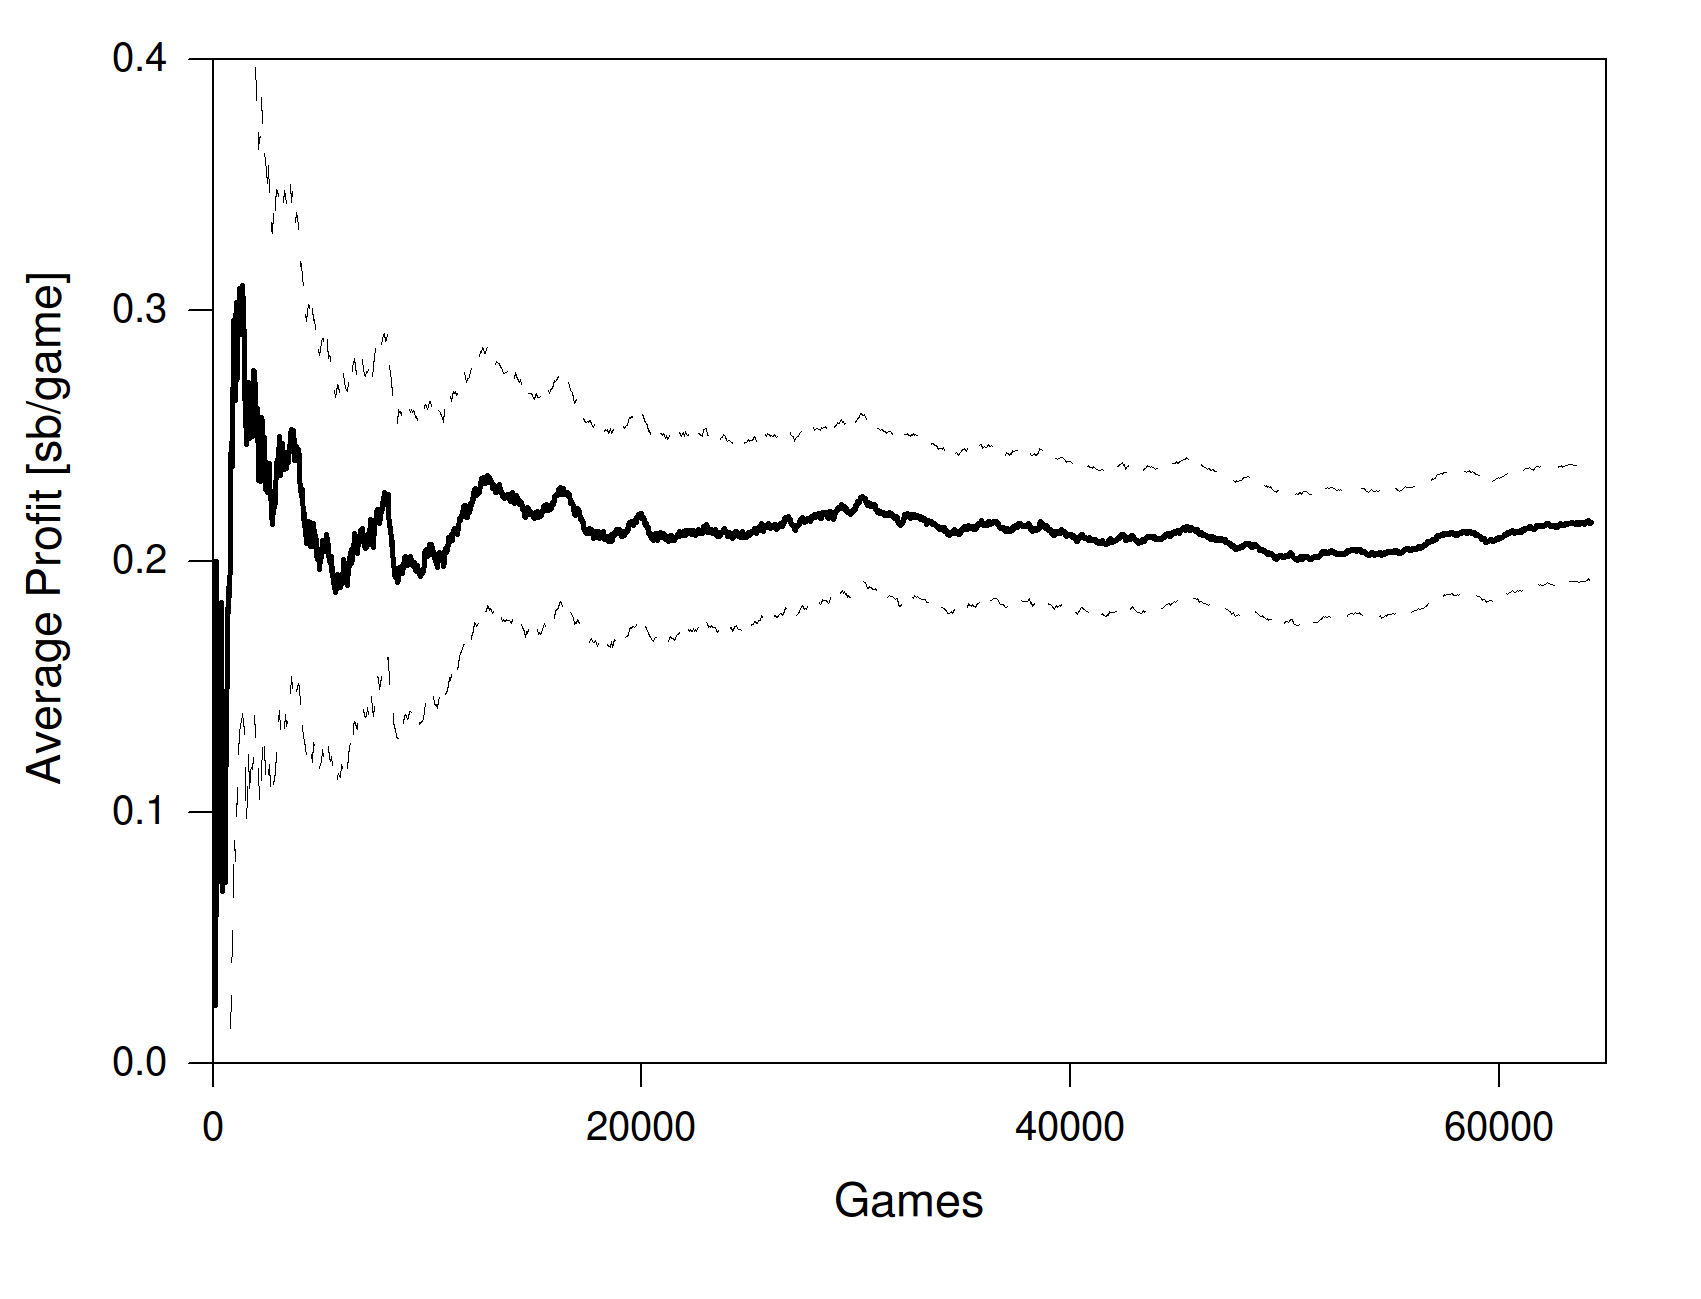
\includegraphics[width=144mm]{Graphs/SBvMB-600-65k-v2.png}
\caption{\mbt Vs. \sbt{} - 65,000 games with default parameters.}
\end{figure}

%From looking at this graph, there doesn't appear to be a whole lot of change after about the 20,000 mark. 
%It's also worth noting the scale on the left, 
%Based on this, I plan to play out 20,000 games (for each variant) in the following experiments. However I may do less if it becomes obvious that it is not needed.

There seems to be little change after 20,000 games. Based on this, I planned to play out 20,000 games (for each variant) in the following experiments\footnote{Again, if I had more time then I would take a much more thorough approach. However, it can take over 24 hours to play out 20,000 games and so playing more is simply not practical.}.



\section{Varying Thinking Time}					% ----

% Want to see if there is a difference.
% Want to see how much of a difference there is. 
% Want to see if there is a simple model to describe the profit as a function of thinking time. 
% How much was I varying thinking time by?
% What was I not varying?
% My predictions?


%From the literature on MCTS and from my experience so far, I expect the performance to increase as thinking time increases. What I don't know is how much the performance will increase by. I doubt it would be a simple relationship since the program is incredibly complex. 

%I predict that, at very high thinking times, the performance will level out to a constant-ish value. I think this because no matter how good \mbts decisions are, its profit is still limited by the rules of poker and by \sbts play style. I also think that the performance will not decrease as the thinking time increases. I think this because the MCTS algorithm is relatively stable and should always reach a point where its answer will not change. At very low thinking times, I'm not sure exactly what will happen. I think there could be a point where \mbt starts to lose to \sbt but I don't know when that will be.

From the literature on MCTS and from my experience so far, I expected the average profit to increase as thinking time increases. I also expected the average profit to eventually level out. This is because no matter how good \mbts decisions are, its profit is still limited by the rules of poker and by \sbts play style. 

To test the effects of thinking time on performance, I ran five trials of 20,000 games each. The only variable I changed was the amount of thinking time given to the MCTS algorithm. 
%I will use the default thinking time, 600ms, as well as 2400ms, 150ms, 38ms and 9ms. I have chosen these values because I think they represent a wide range of abilities for the MCTS algorithm. 
I used the default thinking time (600ms) as well as four times the default (2400ms), one quarter of the default (150ms), one sixteenth of the default (38ms) and one sixty fourth of the default (9ms). I chose those values because I think they represent a wide range of abilities for the MCTS algorithm. 

Here is a graph showing the average profit for the five different thinking times. The error bars are drawn at two times the standard error from the mean. Also note that time is on a log scale.
\begin{figure}[H]
\centering
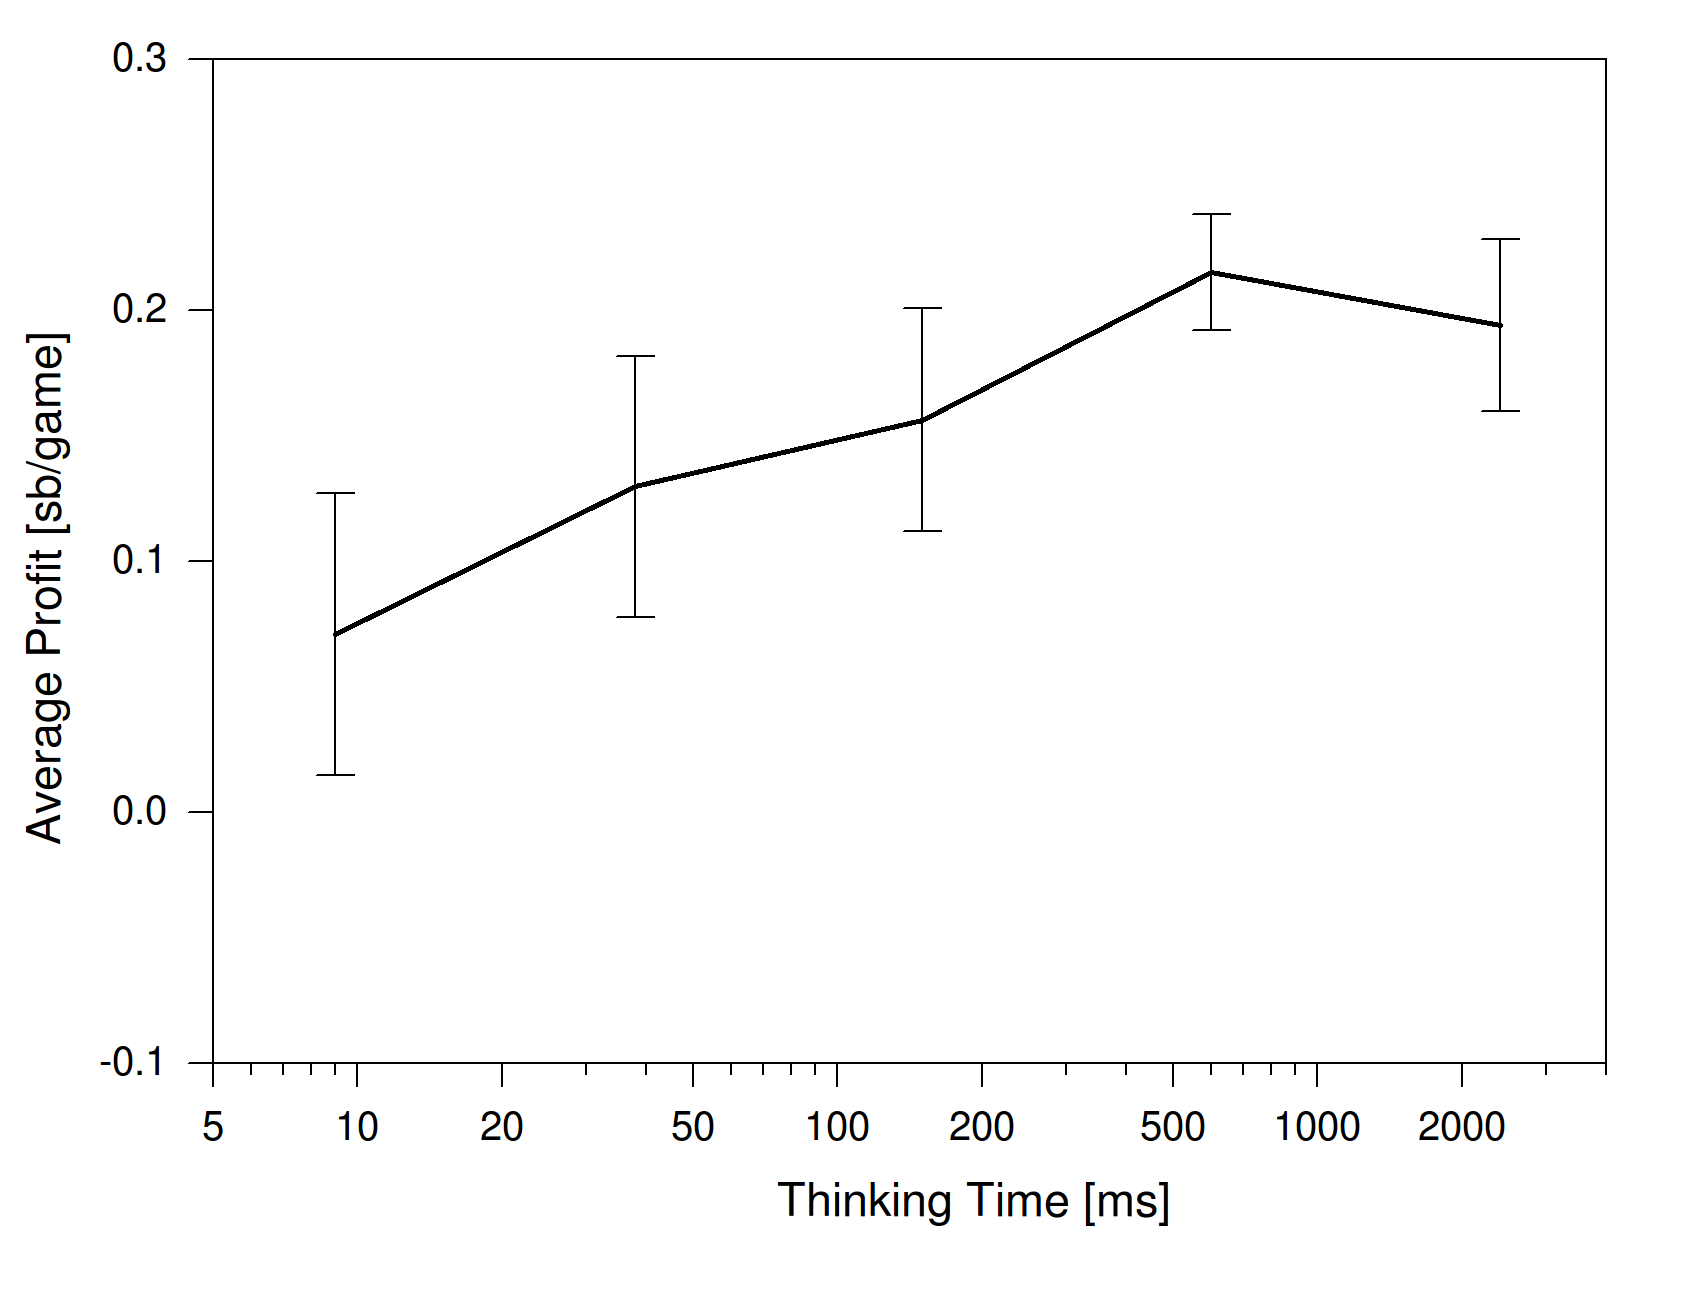
\includegraphics[width=144mm]{Graphs/SBvMB-time.png}
\caption{Average profit of \mbt against \sbt \\ with different thinking times.}
%\label{}
\end{figure}

%From these results, I think it clear that the thinking time does in fact have a significant effect on the average profit. 

I think it is clear from these results that increasing the thinking time has a positive effect on the average profit. 

At 2400ms thinking time, the average profit is slightly lower than at 600ms. Given that both means lie within the error bars of the other, it is most likely due to chance\footnote{However, it could also be caused by something else. If I had more time, I would investigate this further.}. 





\section{Varying Opponent Models}				% ----

One of the original questions I wanted to answer was: how much of an effect do the opponent models have? To find out, I played \mbt against \sbt using all four combinations of the two opponent models, that is: both of them, just the hand rank opponent model, just the next move opponent model and neither of them. 

Note that when I say an opponent model is not being used, I mean that I am using the basic model instead of the one using Weka classifiers. The basic hand rank opponent model is the one which randomly deals the opponent some hole cards and sees who has the best hand. The basic next move opponent model is the one which assigns a probability of \(1 \over 3\) to each of the possible moves\footnote{A basic model which returned different probabilities might perform slightly better. I did briefly experiment with using different probabilities, however it still did not perform very well.}.
%was still no where near as good as the opponent model using Weka.}.
%I obviously expect the trial using both opponent models to do best. I also think that the the trial using only the next move model will do better than the one using only the hand rank opponent model. I think this because 


%Here is a bar chart displaying the average profit with the four different combinations of opponent models.
Here is a bar chart displaying the results, the error bars are drawn at two times the standard error from the mean\footnote{Note that the no-models and hrom-only results were attained after only 5000 games. This was due to time constraints.}.
\begin{figure}[H]
\centering
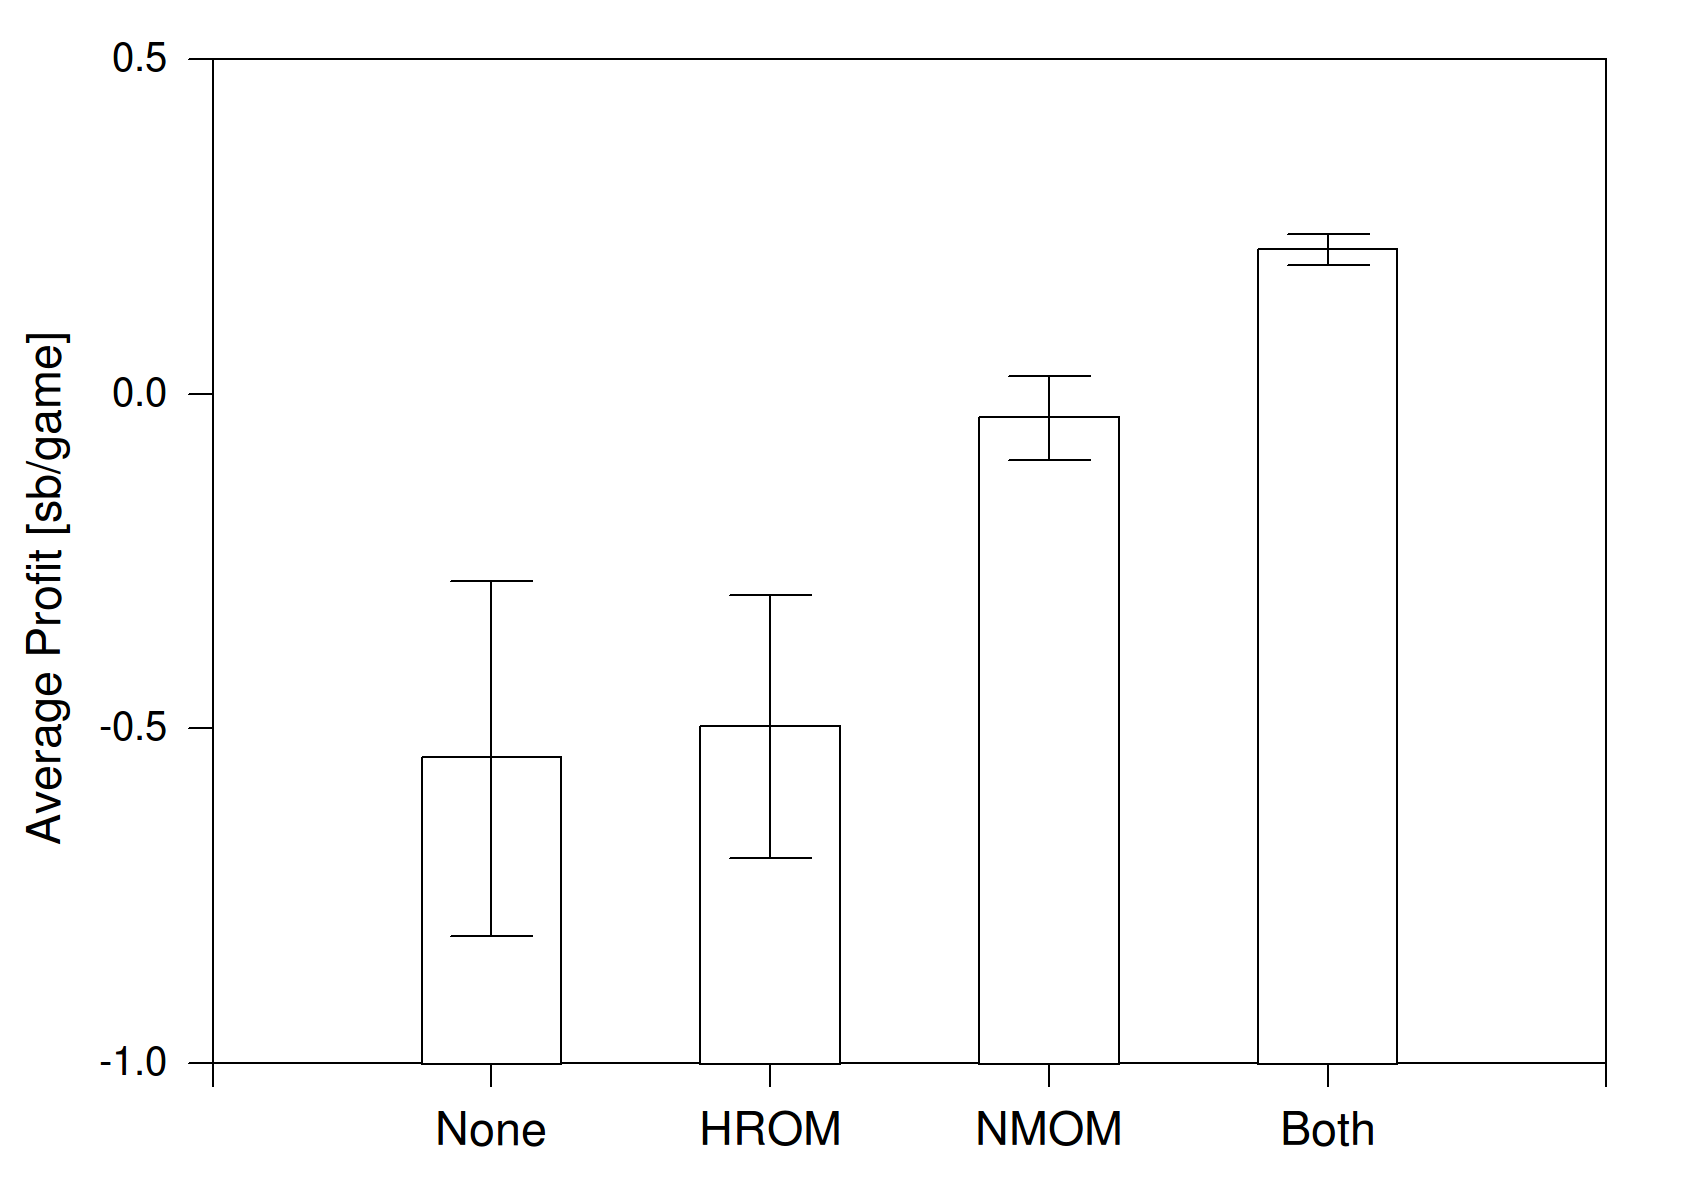
\includegraphics[width=144mm]{Graphs/SBvMB-oppmodels-v2.png}
\caption{Average profit of \mbt against \sbt \\ with different combinations of opponent models.}
%\label{}
\end{figure}

The graph shows that using both opponent models is far superior to any other combination. In fact it is the only combination which actually makes a positive average profit.
%Using only the next move opponent model produces a much higher average profit than using only the hand rank opponent model or no opponent models. 
Using only the next move opponent model is the next best, almost managing to break even. The other two combinations both perform equally poorly.


I think these results show that both opponent models clearly benefit the program and that the next move opponent model is more beneficial than the hand rank opponent model.
%\footnote{Which is consistent with my expectations.}. 





\section{Varying Selection Strategies}			% ----

When dealing with \choices, there are two possible selection strategies, UCT and UCTVar. 
%From early testing, I remember the UCTVar strategy giving a slight increase in performance. 
%I predict that the UCTVar strategy will still do slightly better, although I don't know how much better. 
Here is a bar chart showing the average profit for each strategy. Note that I used \(C = 10\) for the UCT strategy and \(C_1 = 10\) and \(C_2 = 0.1\) for the UCTVar strategy. The error bars are drawn at two times the standard error from the mean.
\begin{figure}[H]
\centering
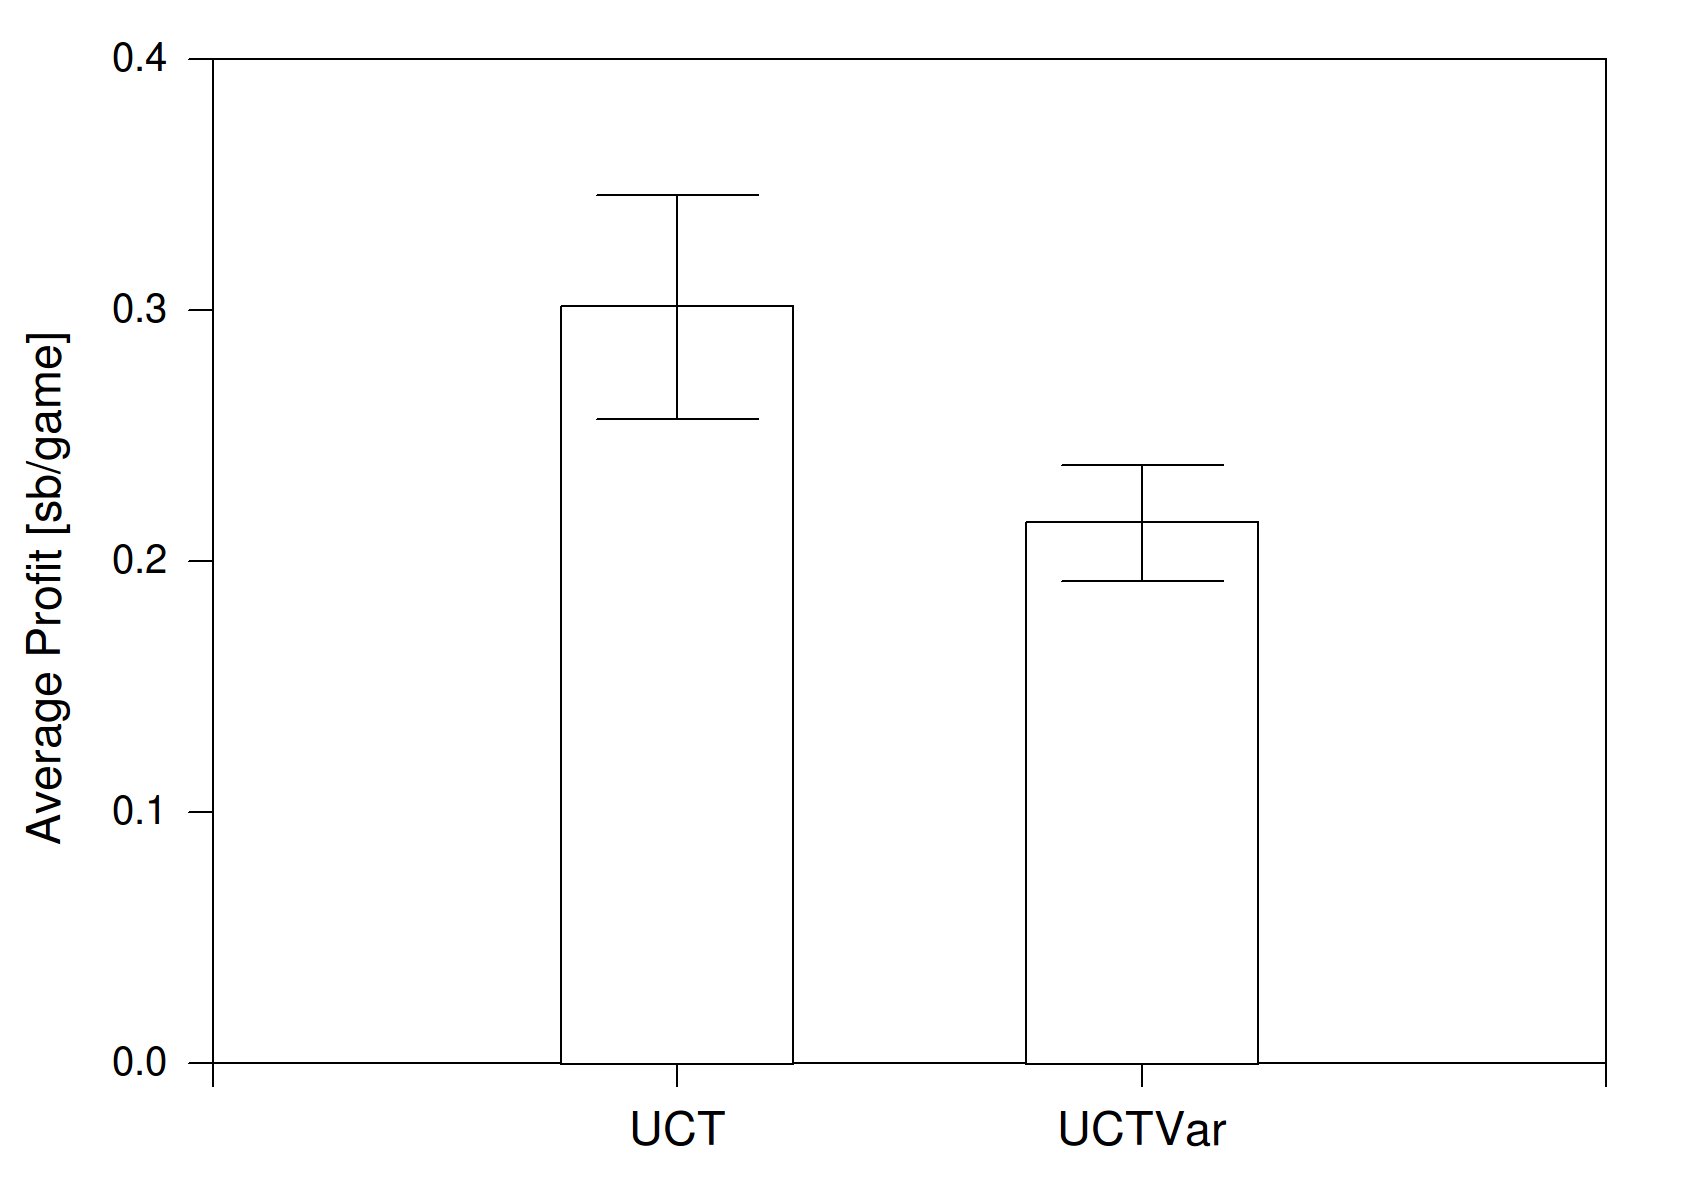
\includegraphics[width=144mm]{Graphs/SBvMB-UCT.png}
\caption{Average profit of \mbt against \sbt \\ with the UCT and UCTVar selection strategies.}
%\label{}
\end{figure}

The results clearly show that the UCT strategy is performing significantly better than the UCTVar strategy. This is exactly the opposite of what I expected\footnote{I am not sure how to explain this, especially as I remember the UCTVar strategy performing better in early testing. I think I might have inadvertently fixed a crippling bug in between testing the two strategies, which made me think that the UCTVar strategy was increasing the performance.}.

The reason for this might be that I am not using the best possible constants. I may also have implemented the UCTVar strategy incorrectly or there could be bugs in the code. All I can say is that, in my implementation, the UCT strategy is superior to the UCTVar strategy.



\section{Varying the Number of Opponents}		% ----

Another one of the original questions that I wanted to answer was: what effect does increasing the number of opponents have? 
%In this section I will try to answer that question. 
There are several things to consider.
%when increasing the number of opponents. 
The first is that, when there are more opponents, there is a lower probability that \mbt will have the best hand\footnote{In fact you would expect the probability to be \(1 \over n\) where \(n\) is the total number of players in the game.}. The second is that the MCTS algorithm does not explicitly take into account the fact that when an opponent does stay in the game, they are more likely to have a better hand than if they had made the same actions in a game with fewer players. This is because the opponent model was trained on data from two player games only. Also, since there are more players in the game, there will be a greater number of branches in the game tree and so the MCTS algorithm will have less time to search through each one. 

On the other hand, you could argue that \mbt has more opportunities to win money through superior play. However, I was still expecting \mbts average profit to decrease as the number of opponents increases. 

The following graph shows the average profit of \mbt when played against one, two, three and four separate instances of \sbt in \pap. Error bars are drawn at two times the standard error from the mean.
\begin{figure}[H]
\centering
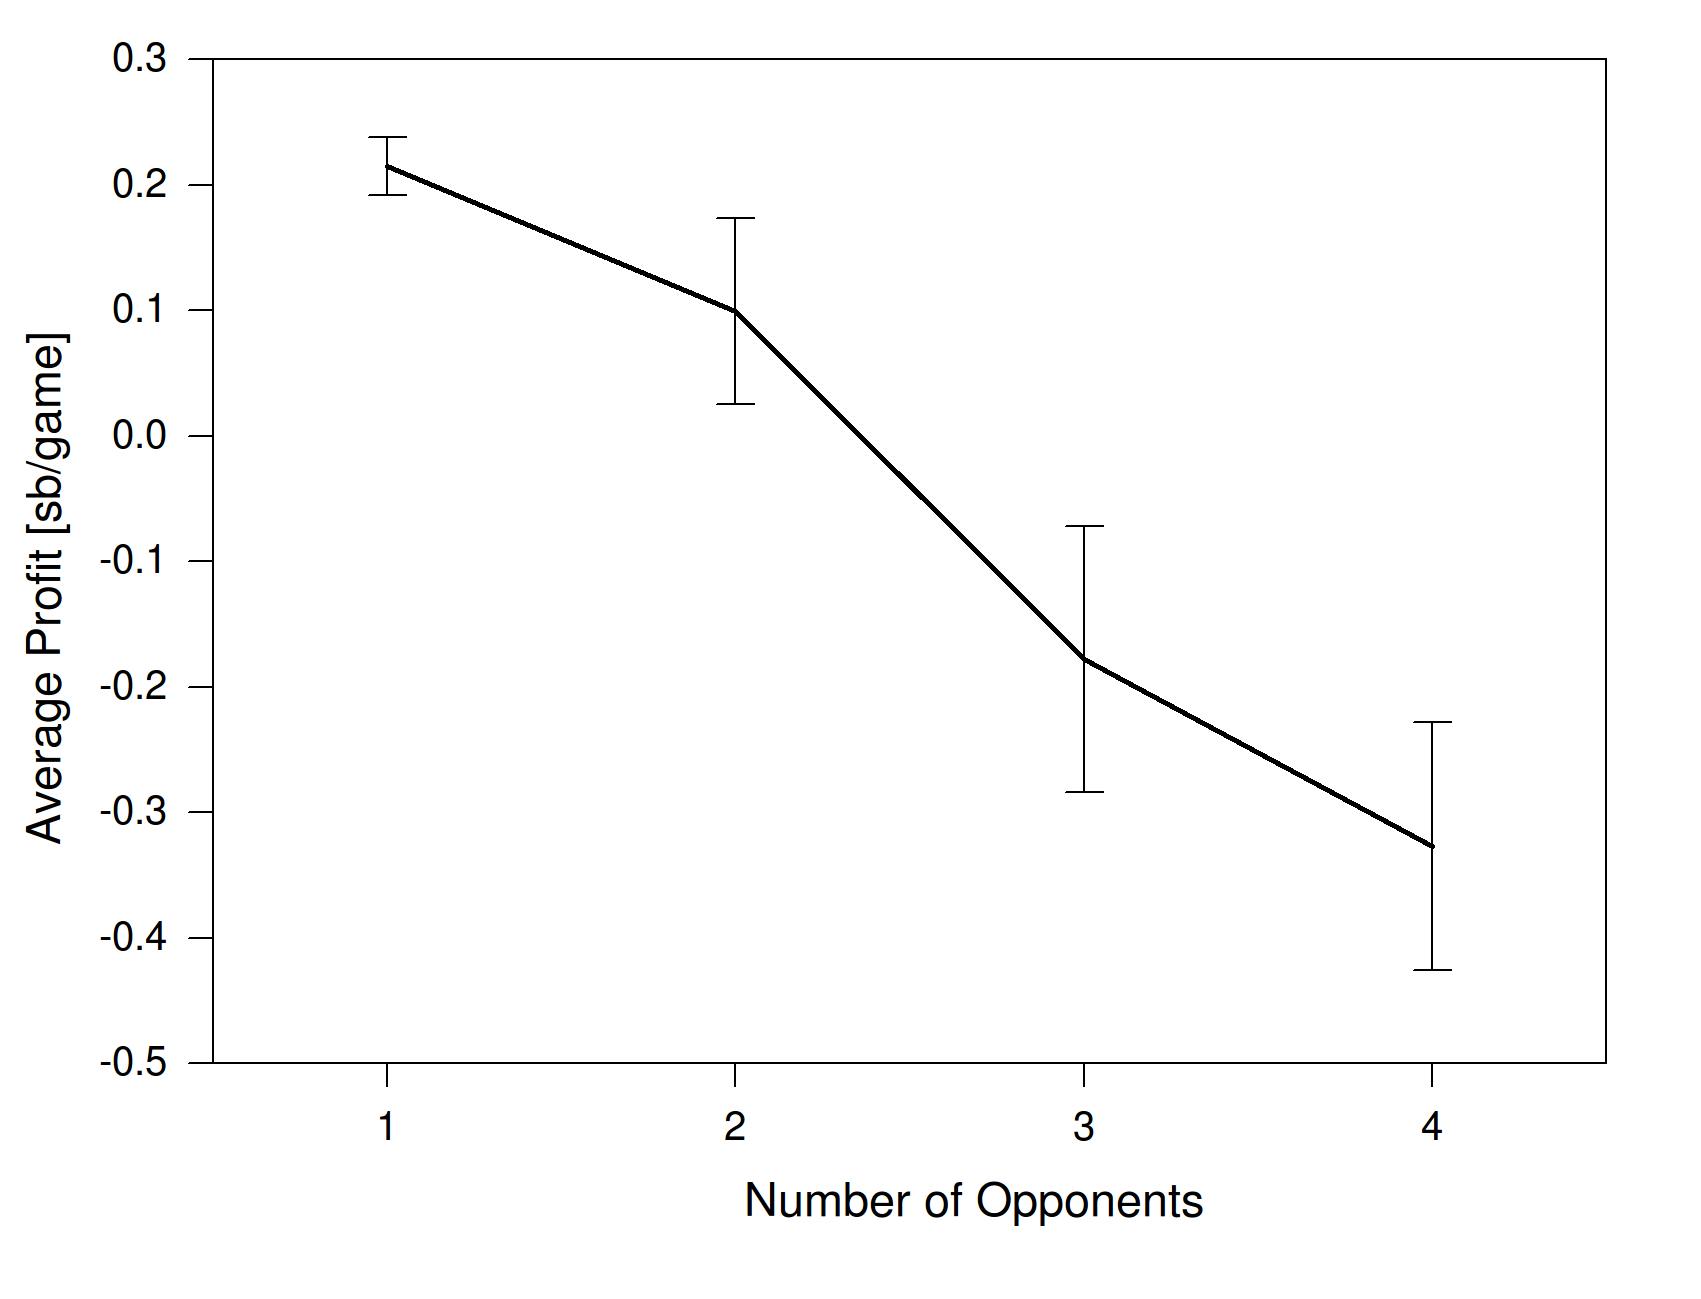
\includegraphics[width=144mm]{Graphs/SBvMB-num.png}
\caption{Average profit of \mbt \\ when played against multiple instances of \sbt.}
%\label{}
\end{figure}

As you can see, the average profit steeply decreases as the number of opponents increases. \mbt is able to make a positive average profit when played against one or two opponents but not when played against three of four. 
%This is consistent with my expectations. 




One of my original success criteria was for \mbt to be able to make the most money when played against three separate instances of \sbt. In the above experiment, \mbt did not achieve this. However, I now know that the default settings I have been using are not optimal. I wanted to complete all of my original success criteria so I attempted to tweak the parameters of \mbt to increase its performance. 

I decided to use the UCT selection strategy (with \(C = 10\)) instead of the UCTVar selection strategy. I also gave the MCTS algorithm 1000ms thinking time instead of 600ms. The following graph shows the average profit of \mbt and all three of the instances of \sbt.
\begin{figure}[H]
\centering
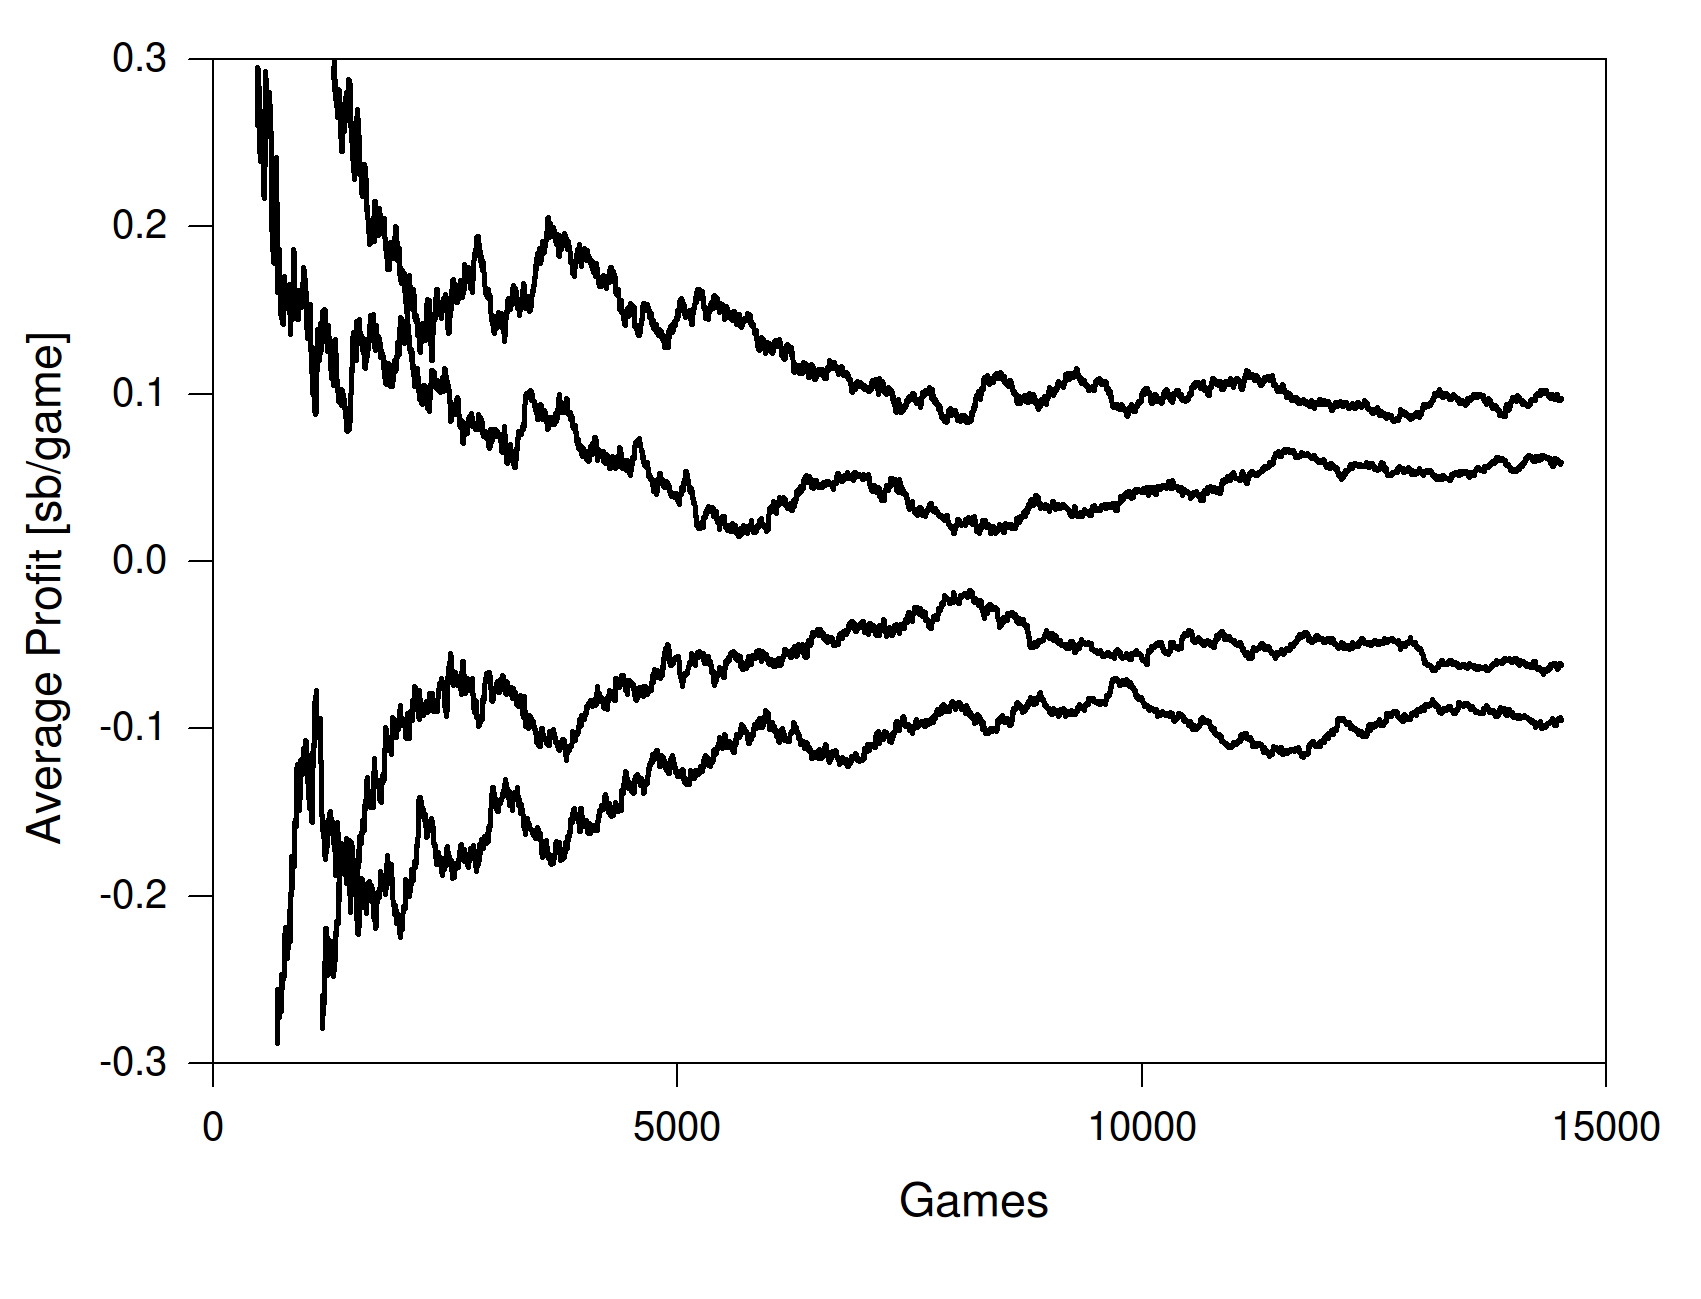
\includegraphics[width=144mm]{Graphs/SBvMB-x3.png}
\caption{Average profit of \mbt and three instances of \sbt \\ over the course of about 15,000 games.}
%\label{}
\end{figure}

The top line is \mbts average profit, 
%the line below that is \sbt{}3's average profit, the line below that is \sbt{}2's average profit and the bottom line is \sbt{}1's average profit. 
the three lines below that are the average profits of the three instances of \sbt\footnote{In my opinion, this shows that \mbt can make the most money when played against three instances of \sbt. If I had more time, I would play more games and try to show this more conclusively.}.

An interesting thing to note is that the \sbt which was sitting to the right of \mbt, seems to be doing much better than the other two instances of \sbt. I have noticed this every time I have played games with multiple opponents. I think this could be due to a situation in which \mbt has a bad hand but gets drawn into the next round with the player to its right just because it is on the big blind.

% Add footnote saying if I had more time...



\section{Other Opponents}						% ----

I originally chose \sbt because it was simple yet still challenging. However, I think it would be interesting to see how my program fares against some other poker bots. 
%In this section, I will play \mbt against some of the other poker bots included with \pap.

Here is a table showing the average profit of \mbt when played against the opponents included in \pap{}\footnote{Note that due to time constraints, I was only able to play about 3000 games for each opponent.}.
\begin{center}
\begin{tabular}{c|c}
Opponent & Average Profit \\
\hline
%\sbt & +0.21 sb/game \\
Simbot & +0.39 sb/game \\
Jagbot & +0.22 sb/game \\
Pokibot & -0.75 sb/game \\
Sparbot & -0.75 sb/game \\
Vexbot & -1.75 sb/game \\
\end{tabular}
\end{center}

\mbt appears to perform well against Simbot and Jagbot, poorly against Pokibot and Sparbot and extremely poorly against Vexbot. I think this shows that, when designing a poker bot, it is important to test against a wide variety of opponents because some strategies may be effective against some opponents and ineffective against others.



Note that \mbt is using the default parameters, including the opponent models trained on the \sbt Vs. \sbt hand histories. This means that a lot of \mbts strategy is specific to \sbt. I have observed that Vexbot in particular seems to exhibit behaviours which \sbt does not. For example, sustained attempts at bluffing. I think that if I were to implement a more general opponent model, it would increase \mbts playing ability when facing other opponents.



%As you can see, \mbt isn't doing too well. I think this is mostly due to the fact that it is still using the opponent models trained on the \sbt Vs. \sbt hand histories. I have observed that Vexbot in particular seems to exhibit behaviours which \sbt does not. For example, sustained attempts at bluffing. 

% Add this to the conclusion
%I think that, if I had more time, I might be able to tweak \mbt to perform better. I also think that I could create a more general opponent model, capable of more accurately predicting the actions of other opponents and maybe even adapting to different opponents on the fly. Alas, I do not have time to complete any of those extensions.




%\section{Profit Distribution}					% ****

%TODO


%\section{General Notes on \mbts Play Style}		% ****

%In this section, I will briefly give some of my thoughts about \mbts play style when facing \sbt. 

%TODO: or put in the conclusion?




%\section{Summary}								% ****


%TODO: or don't bother and just do it in the conclusion

